\subsection{MEX 0-1b: Three-Point fracture toughness test, Opalinus Clay}

Participating institutions of MEX 0-1b (see section \ref{sec:mex01b}): CAU, UFZ

\begin{table}[ht!]
\caption{MEX 0-1b: Data overview}
\label{tab:dms-mex01b-overview}
\small
\begin{tabular}{l|l|l|l|L{4.7cm}}
\hline
\rowcolor{cyan}
Type & Spec. & Owner & Access     & Comment                       \\ 
\hline
EXP  &   Ben    & CAU   & Open    & Output files are uploaded     \\
\hline \hline
MOD  & LEM   & CAU   & Open       & Executable MATLAB P-file      \\
     &       &       & Open       & Input files will be uploaded  \\
\hline
MOD  & FEM   & UFZ   & Open       & Branch to be merged into OGS  \\
     &       &       & Open       & Input files available         \\
%
\hline
\end{tabular}
\end{table}
\normalsize

\subsubsection*{CAU Kiel}

The experimental results of the three-point fracture toughness test on the Opalinus Clay samples are uploaded to the IfG (Kiel) NextCloud server. The data is accessible through the following link:\\
\url{https://nextcloud.ifg.uni-kiel.de/index.php/s/pJxp2eNEJb6PfiS}

The data set, which includes the time, applied force ($N$) and the displacement of the sample at the loading point ($mm$), is provided in a *.txt file. The crack mouth opening displacement (CMOD), which is determined from the image processing technique (section \ref {sec:Fracture_Toughness_Exp}), is given in a *.xlsx file. The data includes the time and the calculated CMOD (mm). 

The required LEM code and the input variables of the three-Point fracture toughness test on the Opalinus Clay samples are uploaded to the IfG (Kiel) NextCloud server. The data is accessible through the following link:\\
\url{https://nextcloud.ifg.uni-kiel.de/index.php/s/ZBFN2rSZ99kPY9M}

The uploaded protected MATLAB file in a *.p format requires a MATLAB version with a built-in Voronoi Tessellation and Delaunay Triangulation functions. The input variables are prepared in two different files for a parallel and perpendicular embedded layer orientations. Figure \ref{fig:Amir_ME1_LEM_Claystone_Data} shows the comparison between the experimental and numerical data as described in section \ref {sec:mex01b}.

\begin{figure}[!ht]
\centering
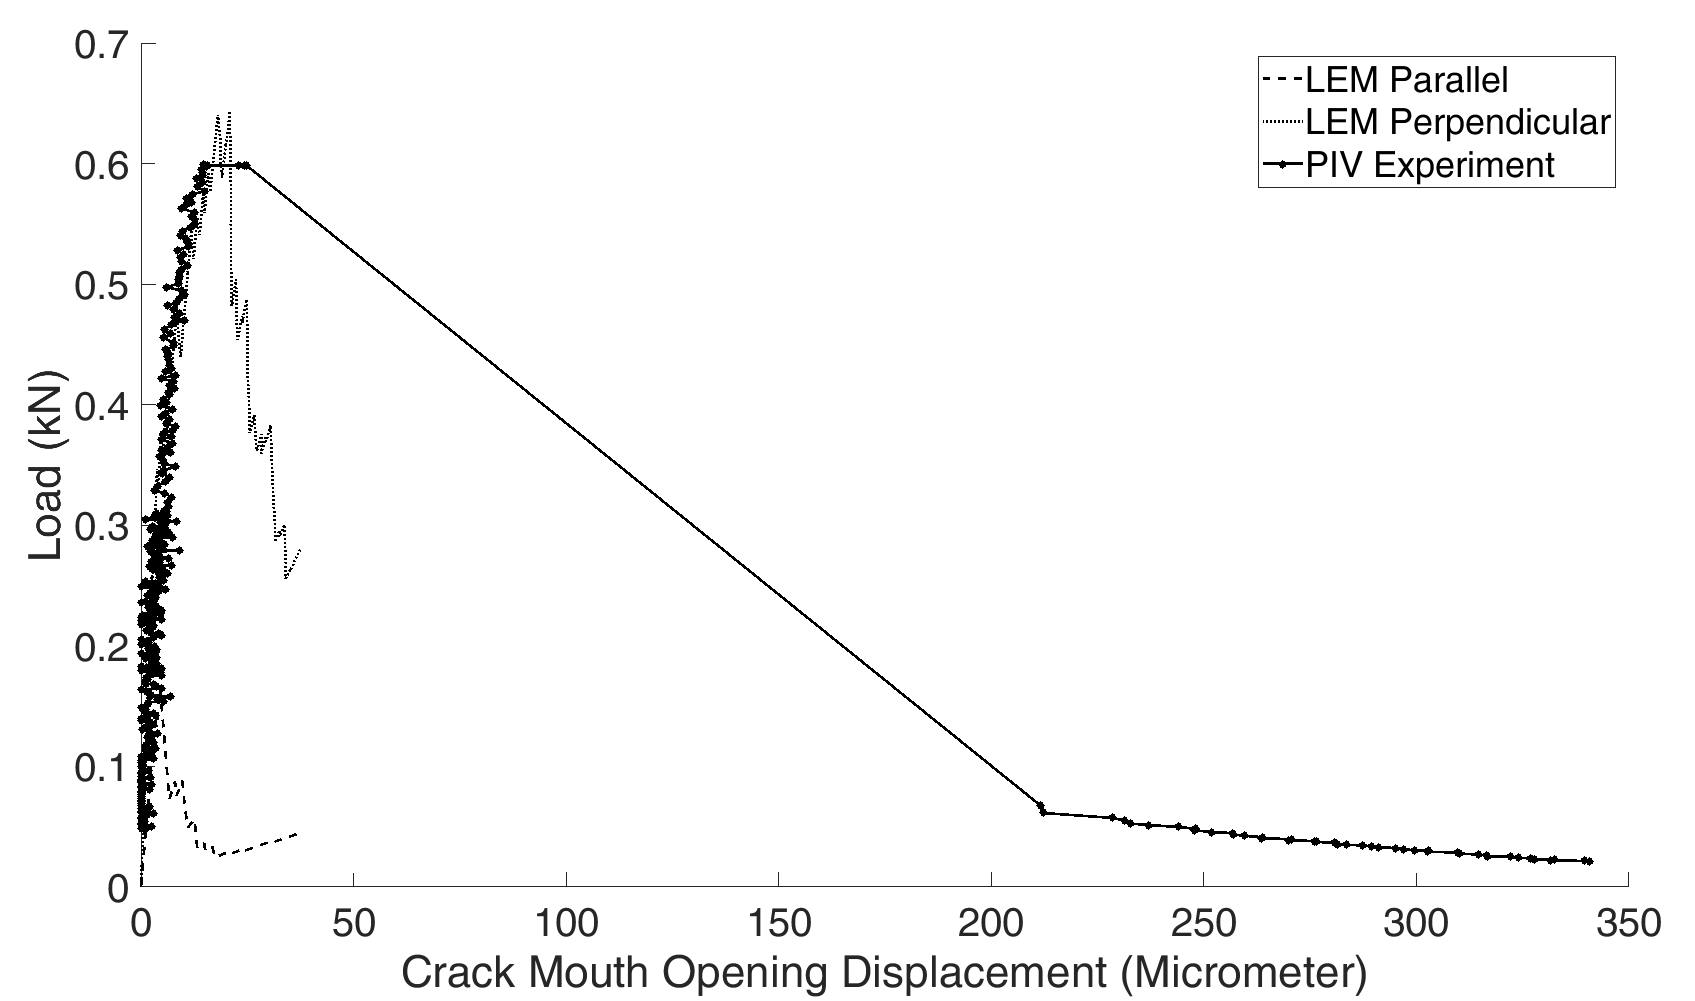
\includegraphics[width=0.75\textwidth]{figures/Amir_ME1_LEM_Claystone_Data.png}
\caption{The load vs. crack mouth opening displacement (CMOD) response of the Opalinus Clay}
\label{fig:Amir_ME1_LEM_Claystone_Data}
\end{figure}

\subsubsection*{UFZ}
The input files for OGS, which were used to simulate the three point bending test performed on the orthogonal and parallel laminations of Opalinus Clay samples, have been uploaded.
The files include the unstructured finite element mesh files in vtu format and OGS input files in xml format.
Also in the mesh files, the material properties are defined per element. 
Particularly for the orthogonal and the parallel Lamentations in the samples are represented through a contrast in the fracture toughness in the samples and can be found in the mesh files.
The load and crack mouth opening displacment computed from the simulations are shown in~\ref{fig:Keita_ME1_VPF_Claystone} as described in section \ref {sec:mex01b}.

\begin{figure}[!ht]
\centering
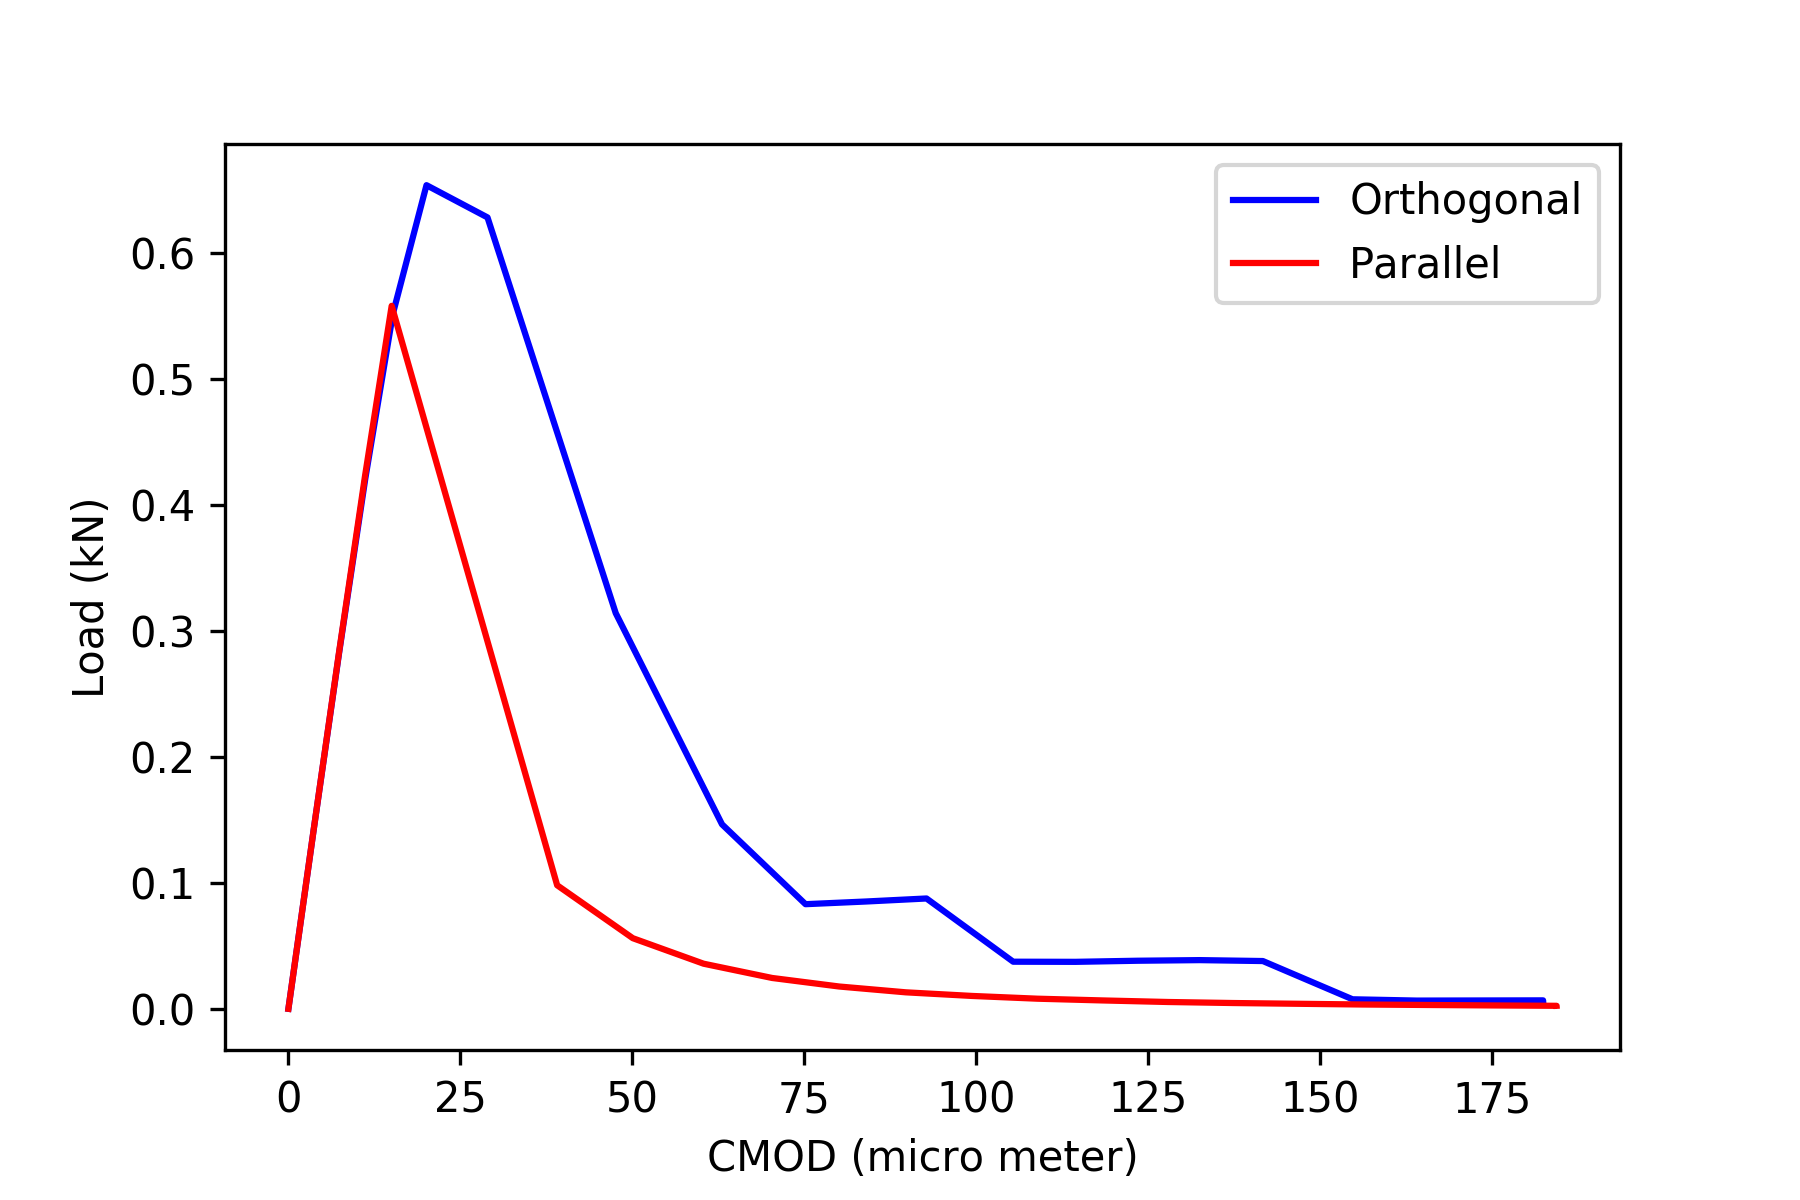
\includegraphics[width=0.75\textwidth]{figures/VPF_ME1_ex_NF_CMOD.png}
\caption{The load vs. crack mouth opening displacement (CMOD) response simulations for orthogonal and parallel lamination by VPF.}
\label{fig:Keita_ME1_VPF_Claystone}
\end{figure}

MEX 0-1b (UFZ) will be also provided as an OGS benchmark case at:\\
\small
\url{www.opengeosys.org/docs/benchmarks/phase-field/phasefield/pf_tpb_ani}
\normalsize

\clearpage
%---------------------------------------------------------
\subsubsection*{Meta Data Overview (according to Dublin Core)}
%---------------------------------------------------------

\begin{table}[!ht]
\caption{MEX 0-1b (CAU)}
\label{tab:dms-mex0-1b}
\small
\begin{tabular}{R{3.5cm}|L{7.5cm}}
\hline
%
Data label & GeomInt, MEX 0-1b, CAU, Bending fracture test, Opalinus Clay \\
URL (Experiments) & \url{https://nextcloud.ifg.uni-kiel.de/index.php/s/pJxp2eNEJb6PfiS} \\
URL (Numerics) & \url{https://nextcloud.ifg.uni-kiel.de/index.php/s/ZBFN2rSZ99kPY9M} \\
Subject  &  Bending fracture test, Opalinus Claye\\
Type of data  &  Experimental data, executable MATLAB P-file, input parameters\\
Subject  &  Bending fracture test, Opalinus Clay\\
Type of data  &  Experimental data, executable MATLAB P-file, input parameters\\
Data quality  &  Quality assured data \\
Status of data  &  Unprocessed data\\
Data format  & txt, xlsx, MATLAB executable P-file\\
Creators  &  Kiel University, Institute of Geomechanics and Geotechnics, Ludewig-Meyn-Stra\ss e 10, 24118, Kiel\\
Source/Origin & In-house code \\
Publisher  &  Kiel University, Institute of Geomechanics and Geotechnics, Ludewig-Meyn-Stra\ss e 10, 24118, Kiel \\
Rights holders &  Kiel University, Institute of Geomechanics and Geotechnics, Ludewig-Meyn-Stra\ss e 10, 24118, Kiel \\
Contributors &   Kiel University, Institute of Geomechanics and Geotechnics: Amir Shoarian Sattari, Frank Wuttke\\
Time/period of creation &  2018-2019\\
Language of the content &  English\\
Update policy &  Stored data is final\\
Access permissions & Full access\\
%
\hline
\end{tabular}
\end{table}

\begin{table}[!ht]
\caption{MEX 0-1b (UFZ)}
\label{tab:dms-mex0-1a}
\small
\begin{tabular}{R{3.5cm}|L{7.5cm}}
\hline
%
Data label & MEX 0-1b (UFZ) \\
URL & \url{www.opengeosys.org/docs/benchmarks/phase-field/phasefield/} \\ 
Subject  & Bending fracture test, Opalinus Clay \\
Type of data  & Data set (structured data in a defined format) \\
Data quality  & Quality assured data by benchmarking \\
Status of data  & Processed data \\
Data format  & OGS files \\
Creators  & Yoshioka, Keita  \\
Source/Origin & Open source \\
Publisher  & Helmholtz Centre for Environmental Research UFZ \\
Rights holders & Helmholtz Centre for Environmental Research UFZ \\
Contributors & Yoshioka, Keita \\
Time/period of creation & 2019-2020 \\
Language of content & English \\
Update policy & To be merged to OGS benchmarks (see below) \\
Access permissions & Free access \\
%
\hline
\end{tabular}
\end{table}
